

\section{Aprendizaje Supervisado}

La esencia del aprendizaje automático supervisado es la creación de mecanismos que puedan examinar ejemplos y producir generalizaciones \cite{goldberg2017neural}. Diseñamos un algoritmo cuya entrada es un conjunto de ejemplos etiquetados y cuya salida es una función (o un programa) que recibe una instancia y produce la etiqueta deseada. Por ejemplo, si la tarea es distinguir entre correos electrónicos de spam y no spam, los ejemplos etiquetados serían correos electrónicos etiquetados como spam y correos electrónicos etiquetados como no spam. Se espera que la función resultante produzca predicciones de etiquetas correctas también para instancias que no ha visto durante el entrenamiento. Este enfoque difiere de diseñar un algoritmo para realizar la tarea (por ejemplo, sistemas basados en reglas diseñados manualmente).

\subsection{Funciones Parametrizadas}

Buscar en el conjunto de todas las posibles funciones es un problema muy difícil (y bastante mal definido) \cite{goldberg2017neural}. A menudo nos limitamos a buscar dentro de familias específicas de funciones. Por ejemplo, el espacio de todas las funciones lineales con $d_{in}$ entradas y $d_{out}$ salidas. Estas familias de funciones se llaman clases de hipótesis. Al restringirnos a una clase de hipótesis específica, estamos inyectando al aprendiz con sesgo inductivo, es decir, un conjunto de suposiciones sobre la forma de la solución deseada. Algunas clases de hipótesis facilitan procedimientos eficientes para buscar la solución.

\section{Modelos Lineales}

Una clase de hipótesis común es la de una función lineal de alta dimensión:

\begin{equation}
\begin{split}
f(\vec{x}) = \vec{x} \cdot W + \vec{b}\\
\vec{x} \in  \mathcal{R}^{d_{in}} & \quad W \in  \mathcal{R}^{d_{in}\times d_{out}} \quad \vec{b} \in  \mathcal{R}^{d_{out}}
\end{split}
\end{equation}

El vector $\vec{x}$ es la entrada de la función. La matriz $W$ y el vector $\vec{b}$ son los parámetros. El objetivo del aprendiz es establecer los valores de los parámetros $W$ y $\vec{b}$ de manera que la función se comporte como se pretende en una colección de valores de entrada $\vec{x}_{1:k} = \vec{x}_1,\dots,\vec{x}_k$ y las correspondientes salidas deseadas $\vec{y}_{1:k} = \vec{y}_1,\dots,\vec{y}_k$. La tarea de buscar en el espacio de funciones se reduce así a buscar en el espacio de parámetros.

\subsection{Ejemplo: Detección de Idiomas}

Consideremos la tarea de distinguir entre documentos escritos en inglés y documentos escritos en alemán. Este es un problema de clasificación binaria:

\begin{equation}
\begin{split}
f(\vec{x}) = \vec{x} \cdot \vec{w} + b
\end{split}
\end{equation}

donde $d_{out} = 1$, donde $\vec{w}$ es un vector y $b$ es un escalar. El rango de la función lineal es $[-\infty, \infty]$. Para usarla en la clasificación binaria, es común pasar la salida de $f(x)$ a través de la función $signo$, mapeando los valores negativos a -1 (clase negativa) y los valores no negativos a +1 (clase positiva).

Las frecuencias de letras son buenos predictores (características) para esta tarea, pero aún más informativos son los recuentos de bigramas de letras, es decir, pares de letras consecutivas. Es probable que nos encontremos con un documento nuevo sin ninguna de las palabras que observamos en el conjunto de entrenamiento, mientras que un documento sin ninguno de los distintivos bigramas de letras es significativamente menos probable \cite{goldberg2017neural}. Supongamos que tenemos un alfabeto de 28 letras (a-z, espacio y un símbolo especial para todos los demás caracteres, incluidos dígitos, puntuación, etc.). Los documentos se representan como vectores de dimensión $28 \times 28$, es decir, $\vec{x} \in \mathcal{R}^{784}$. Cada entrada $\vec{x}_{[i]}$ representa un recuento de una combinación particular de letras en el documento, normalizado por la longitud del documento. Por ejemplo, si denotamos por $\vec{x}_{ab}$ la entrada de $\vec{x}$ correspondiente al bigrama de letras $ab$:

\begin{equation}
\vec{x}_{ab} = \frac{\#ab}{|D|}
\end{equation}

donde $\#ab$ es el número de veces que aparece el bigrama $ab$ en el documento y $|D|$ es el número total de bigramas en el documento (la longitud del documento).

La figura muestra histogramas de bigramas de caracteres para documentos en inglés y alemán. Los guiones bajos representan espacios. Solo se muestran los bigramas de caracteres más frecuentes.

\begin{figure}[htb]
	\centering
	 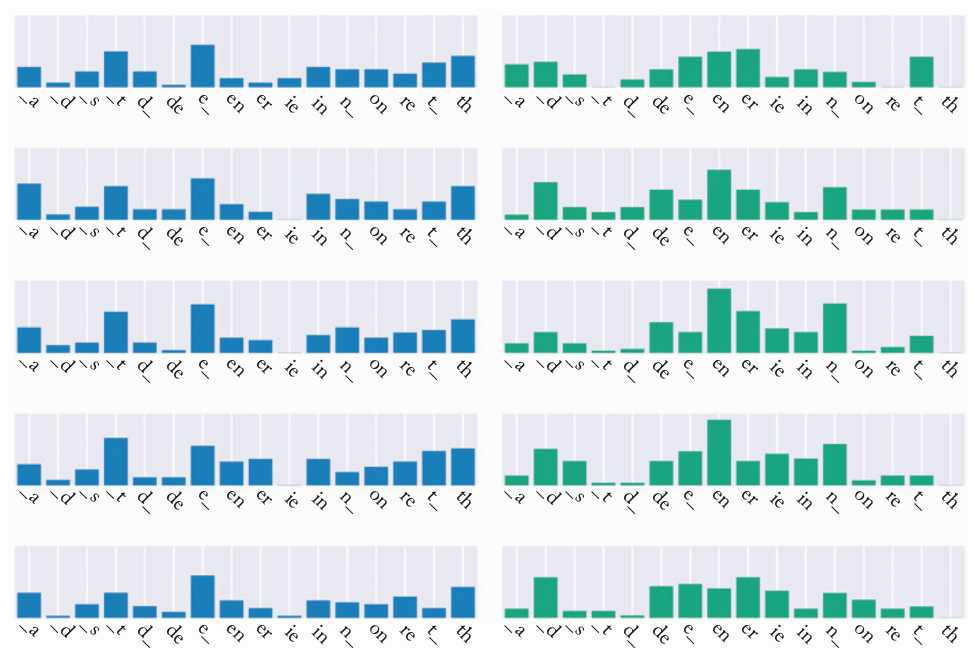
\includegraphics[scale=0.26]{pics/langbigrams.png}
\end{figure}

Fuente: \cite{goldberg2017neural}

La figura anterior muestra patrones claros en los datos. Dado un nuevo elemento, por ejemplo:

\begin{figure}[htb]
	\centering
	 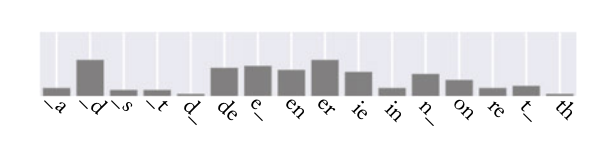
\includegraphics[scale=0.4]{pics/langbigramstest.png}
\end{figure}

Probablemente podríamos decir que es más similar al grupo alemán que al grupo inglés (observar la frecuencia de "th" y "ie"). No podemos usar una regla única definitiva como "si tiene th es inglés" o "si tiene ie es alemán". Aunque los textos en alemán tienen considerablemente menos "th" que el inglés, la combinación "th" puede ocurrir en textos en alemán, al igual que la combinación "ie" puede ocurrir en inglés. La decisión requiere ponderar diferentes factores relativos entre sí.

Podemos formalizar el problema en un entorno de aprendizaje automático utilizando un modelo lineal:

\begin{equation}
\begin{split}
\hat{y} = \text{sign}(\vec{x}\cdot \vec{w} + b) = \text{sign}(\vec{x}_{aa}\times \vec{w}_{aa}+ \vec{x}_{ab}\times \vec{w}_{ab}+ \vec{x}_{ac}\times \vec{w}_{ac} \dots +b)
\end{split}
\end{equation}

Un documento se considerará inglés si $f(\vec{x}) \geq 0$ y alemán en caso contrario. La intuición detrás del aprendizaje es la siguiente:

\begin{enumerate}
\item El aprendizaje debe asignar valores positivos grandes a las entradas de $\vec{w}$ asociadas con pares de letras que son mucho más comunes en inglés que en alemán (por ejemplo, "th").
\item También debe asignar valores negativos a los pares de letras que son mucho más comunes en alemán que en inglés (por ejemplo, "ie", "en").
\item Finalmente, debe asignar valores alrededor de cero a los pares de letras que son comunes o raros en ambos idiomas.
\end{enumerate}


%Translate this Latex book chapter to Spanish. Output in Latex format. Rearrange bullet points (\items) into full paragraphs. Make sure that sentences are connected in a more fluid way as they come.
\section{Clasificación binaria log-lineal}
La salida $f(\vec{x})$ se encuentra en el rango $[-\infty,\infty]$, y la mapeamos a una de las dos clases $\{-1,+1\}$ utilizando la función $signo$. Esto es adecuado si lo único que nos importa es la clase asignada. Sin embargo, puede que también estemos interesados en la confianza de la decisión o en la probabilidad que el clasificador asigna a la clase.

Una alternativa que facilita esto es mapear la salida al rango $[0,1]$ mediante una función de compresión como la función sigmoide $\sigma(x)$:

\begin{equation}
\sigma(x) = \frac{1}{1+e^{-x}}
\end{equation}

lo que resulta en:

\begin{equation}
\hat{y}=\sigma(f(\vec{x})) = \frac{1}{1+e^{-\vec{x}\cdot \vec{w}+b}}
\end{equation}

La función sigmoide es monótona creciente y mapea los valores al rango $[0, 1]$, con $0$ mapeado a $\frac{1}{2}$. Cuando se utiliza con una función de pérdida adecuada (que se discutirá más adelante), las predicciones binarias realizadas mediante el modelo log-lineal se pueden interpretar como estimaciones de la probabilidad de pertenencia a la clase:

\begin{equation}
 \sigma(f(\vec{x})) = P(\hat{y} = 1| \vec{x}) \quad \text{de que $\vec{x}$ pertenezca a la clase positiva.}
\end{equation}

También obtenemos $P(\hat{y} = 0| \vec{x}) = 1 - P(\hat{y} = 1| \vec{x}) = 1-\sigma(f(\vec{x}))$. Cuanto más cercano sea el valor a $0$ o $1$, más seguro está el modelo en su predicción de pertenencia a la clase, y el valor $0.5$ indica incertidumbre del modelo.

\section{Clasificación multiclase}
La mayoría de los problemas de clasificación son de naturaleza multiclase: se asignan ejemplos a una de las $k$ clases diferentes. Por ejemplo, se nos puede dar un documento y se nos pide clasificarlo en uno de los seis posibles idiomas: inglés, francés, alemán, italiano, español y otros.

Una solución posible es considerar seis vectores de pesos $\vec{w}_{EN}$, $\vec{w}_{FR}$, $\dots$ y sesgos (uno para cada idioma). Predecimos el idioma que resulta en el puntaje más alto:

\begin{equation}
 \hat{y} = f(\vec{x}) = \operatorname{argmax}_{L \in \{ EN,FR,GR,IT,SP,O \}} \quad \vec{x}\cdot \vec{w}_L+ b_{L}
\end{equation}

Los seis conjuntos de parámetros $\vec{w}_L \in  \mathcal{R}^{784}$ y $b_L$ se pueden organizar en una matriz $W \in \mathcal{R}^{784\times6}$ y un vector $\vec{b} \in \mathcal R^6$, y la ecuación se puede reescribir como:

\begin{equation}
 \begin{split}
  \vec{\hat{y}} = f(\vec{x}) = \quad & \vec{x} \cdot W + \vec{b}\\
   \text{predicción} = \hat{y} = \quad  & \operatorname{argmax}_i \vec{\hat{y}}_{[i]}
 \end{split}
\end{equation}

Aquí, $\vec{\hat{y}} \in \mathcal{R}^6$ es un vector de los puntajes asignados por el modelo a cada idioma, y determinamos el idioma predicho tomando el argmax sobre las entradas de $\vec{\hat{y}}$ (las columnas con el valor más alto).

\section{Representaciones}
Consideremos el vector $\vec{\hat{y}}$ resultante de aplicar un modelo entrenado a un documento. Podemos considerar que este vector es una representación del documento, ya que captura las propiedades del documento que son importantes para nosotros, es decir, los puntajes de los diferentes idiomas. La representación $\vec{\hat{y}}$ contiene estrictamente más información que la predicción $\operatorname{argmax}_i \vec{\hat{y}}_{[i]}$.

Por ejemplo, $\vec{\hat{y}}$ se puede utilizar para distinguir documentos en los que el idioma principal es el alemán, pero que también contienen una cantidad considerable de palabras en francés. El agrupamiento de documentos basado en $\vec{\hat{y}}$ podría ayudar a descubrir documentos escritos en dialectos regionales o por autores multilingües.

Los vectores $\vec{x}$ que contienen los recuentos normalizados de los bigramas de letras para los documentos también son representaciones de los documentos. Se podría argumentar que contienen un tipo de información similar a los vectores $\vec{\hat{y}}$. Sin embargo, las representaciones en $\vec{\hat{y}}$ son más compactas (6 entradas en lugar de 784) y más especializadas para el objetivo de predicción de idioma. El agrupamiento por los vectores $\vec{x}$ probablemente revelaría similitudes en los documentos que no se deben a una mezcla particular de idiomas, sino tal vez al tema o estilo de escritura del documento.

La matriz entrenada $W \in \mathcal{R}^{784 \times 6}$ también se puede considerar como una representación aprendida. Podemos considerar dos vistas de $W$, como filas o como columnas.

\begin{figure}[htb]
	\centering
	 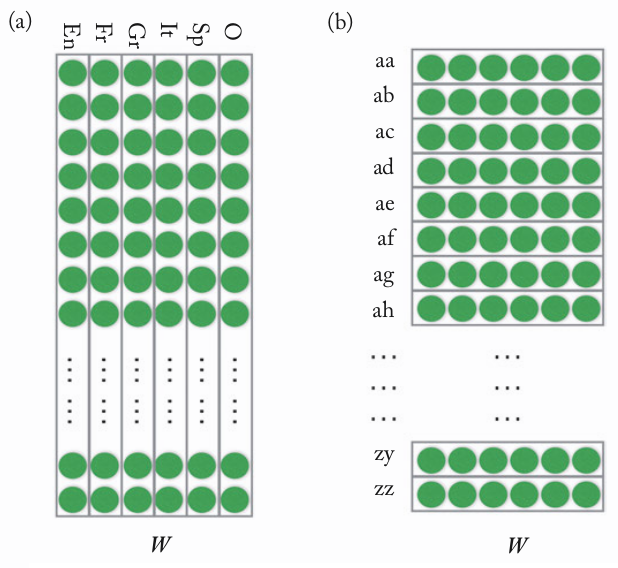
\includegraphics[scale=0.35]{pics/2rep.png}
\end{figure}

Dos vistas de la matriz $W$. (a) Cada columna corresponde a un idioma. (b) Cada fila corresponde a un bigrama de letras. Fuente: \cite{goldberg2017neural}.

Una columna de $W$ puede tomarse como una representación vectorial de $784$ dimensiones de un idioma en términos de sus patrones característicos de bigramas de letras. Luego, podemos agrupar los 6 vectores de idioma según su similitud. Cada una de las 784 filas de $W$ proporciona una representación vectorial de 6 dimensiones de ese bigrama en términos de los idiomas que promueve. Las representaciones son fundamentales para el aprendizaje profundo. Se podría argumentar que el principal poder del aprendizaje profundo es la capacidad de aprender buenas representaciones.

En el caso lineal, las representaciones son interpretables, ya que podemos asignar una interpretación significativa a cada dimensión en el vector de representación. Por ejemplo, cada dimensión puede corresponder a un idioma o a un determinado bigrama de letras.

Por otro lado, los modelos de aprendizaje profundo a menudo aprenden una cascada de representaciones de la entrada que se construyen una encima de la otra. Estas representaciones a menudo no son interpretables, es decir, no sabemos qué propiedades de la entrada capturan. Sin embargo, siguen siendo muy útiles para hacer predicciones.

\section{Representación de Vectores One-Hot}
El vector de entrada $\vec{x}$ en nuestro ejemplo de clasificación de idioma contiene los recuentos normalizados de los bigramas en el documento $D$. Este vector se puede descomponer en un promedio de $|D|$ vectores, cada uno correspondiente a una posición particular del documento $i$:

\begin{equation}
 \vec{x} = \frac{1}{|D|} \sum_{i=1}^{|D|} \vec{x}^{D_{[i]}}
\end{equation}

Aquí, $D_{[i]}$ es el bigrama en la posición $i$ del documento. Cada vector $\vec{x}^{D_{[i]}} \in \mathcal{R}^{784}$ es un vector one-hot, lo que significa que todos los elementos son cero excepto la única entrada que corresponde al bigrama de letras $D_{[i]}$, que es 1. El vector resultante $\vec{x}$ se conoce comúnmente como un promedio de bolsa de bigramas (más generalmente, una bolsa de palabras promediada, o simplemente una bolsa de palabras).

Las representaciones de bolsa de palabras contienen información sobre las identidades de todas las "palabras" (en este caso, bigramas) del documento, sin considerar su orden. Una representación one-hot se puede considerar como una bolsa de una sola "palabra".

\begin{figure}[htb]
	\centering
	 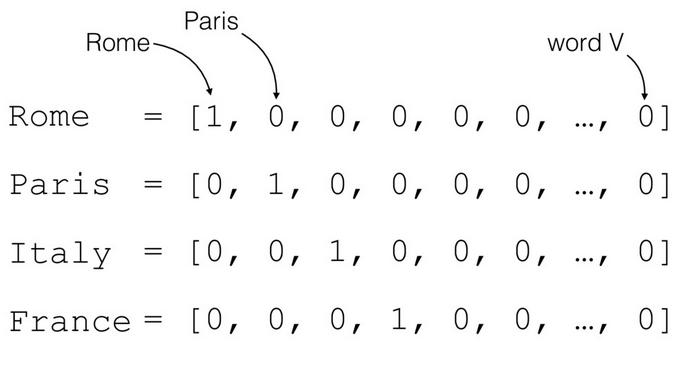
\includegraphics[scale=0.3]{pics/onehot.png}
\end{figure}

Vectores one-hot de palabras.

Fuente: \url{https://medium.com/@athif.shaffy/one-hot-encoding-of-text-b69124bef0a7}.

%Translate this Latex book chapter to Spanish. Output in Latex format. Rearrange bullet points (\items) into full paragraphs. Make sure that sentences are connected in a more fluid way as they come.\section{Clasificación Log-lineal de Múltiples Clases}
En el caso binario, transformamos la predicción lineal en una estimación de probabilidad al pasarla por la función sigmoide, lo que resulta en un modelo log-lineal. En el caso de múltiples clases, el análogo es pasar el vector de puntajes a través de la función \textbf{softmax}:

\begin{equation}
 \operatorname{softmax}(\vec{x})_{[i]} = \frac{e^{\vec{x}_{[i]}}}{\sum_j e^{\vec{x}_{[j]}}}
\end{equation}

Lo que resulta en:

\begin{equation}
\begin{split}
\vec{\hat{y}} \quad & =  \operatorname{softmax}(\vec{x} \cdot W + \vec{b})  \\
\vec{\hat{y}}_{[i]} \quad & = \frac{e^{(\vec{x} \cdot W + \vec{b})_{[i]}}}{\sum_j e^{(\vec{x} \cdot W + \vec{b})_{[j]}}}
\end{split}
\end{equation}

La transformación softmax fuerza a los valores en $\hat{\vec{y}}$ a ser positivos y sumar 1, lo que los hace interpretables como una distribución de probabilidad.

\section{Entrenamiento}
Cuando se entrena una función parametrizada (por ejemplo, un modelo lineal, una red neuronal), se define una función de pérdida $L(\hat{y}, y)$, que establece la pérdida al predecir $\hat{y}$ cuando la salida verdadera es $y$.

\begin{displaymath}
L(f(\vec{x};\Theta), y)
\end{displaymath}

Utilizamos el símbolo $\Theta$ para denotar todos los parámetros del modelo (por ejemplo, $W, \vec{b}$).

El objetivo del entrenamiento es minimizar la pérdida en los diferentes ejemplos de entrenamiento. Formalmente, una función de pérdida $L(\hat{y},y)$ asigna una puntuación numérica (un escalar) a una salida predicha $\hat{y}$ dada la salida esperada verdadera $y$. La función de pérdida debería alcanzar su valor mínimo para los casos en los que la predicción sea correcta.

También podemos definir una pérdida en todo el corpus con respecto a los parámetros $\Theta$ como la pérdida promedio en todos los ejemplos de entrenamiento:

\begin{displaymath}
 \mathcal{L}(\Theta) = \frac{1}{n} \sum_{i=1}^n L(f(\vec{x}_i;\Theta), y_i)
\end{displaymath}

El objetivo del algoritmo de entrenamiento es establecer los valores de los parámetros $\Theta$ de manera que el valor de $\mathcal{L}$ se minimice.

\begin{displaymath}
 \hat{\Theta} = \operatorname{argmin}_{\Theta} \mathcal{L}(\Theta) =  \operatorname{argmin}_{\Theta} \frac{1}{n} \sum_{i=1}^n L(f(\vec{x}_i;\Theta), y_i)
\end{displaymath}

\subsection{Optimización basada en Gradiente}
Las funciones se

entrenan utilizando métodos basados en gradientes. Estos métodos funcionan mediante el cálculo repetido de una estimación de la pérdida $L$ sobre el conjunto de entrenamiento. El método de entrenamiento calcula los gradientes de los parámetros ($\Theta$) con respecto a la estimación de pérdida y mueve los parámetros en la dirección opuesta al gradiente. Los diferentes métodos de optimización difieren en cómo se calcula la estimación de error y cómo se define el movimiento en la dirección opuesta al gradiente.

Si la función es convexa, el óptimo será global. De lo contrario, el proceso solo garantiza encontrar un óptimo local.

\begin{figure}[htb]
	\centering
	 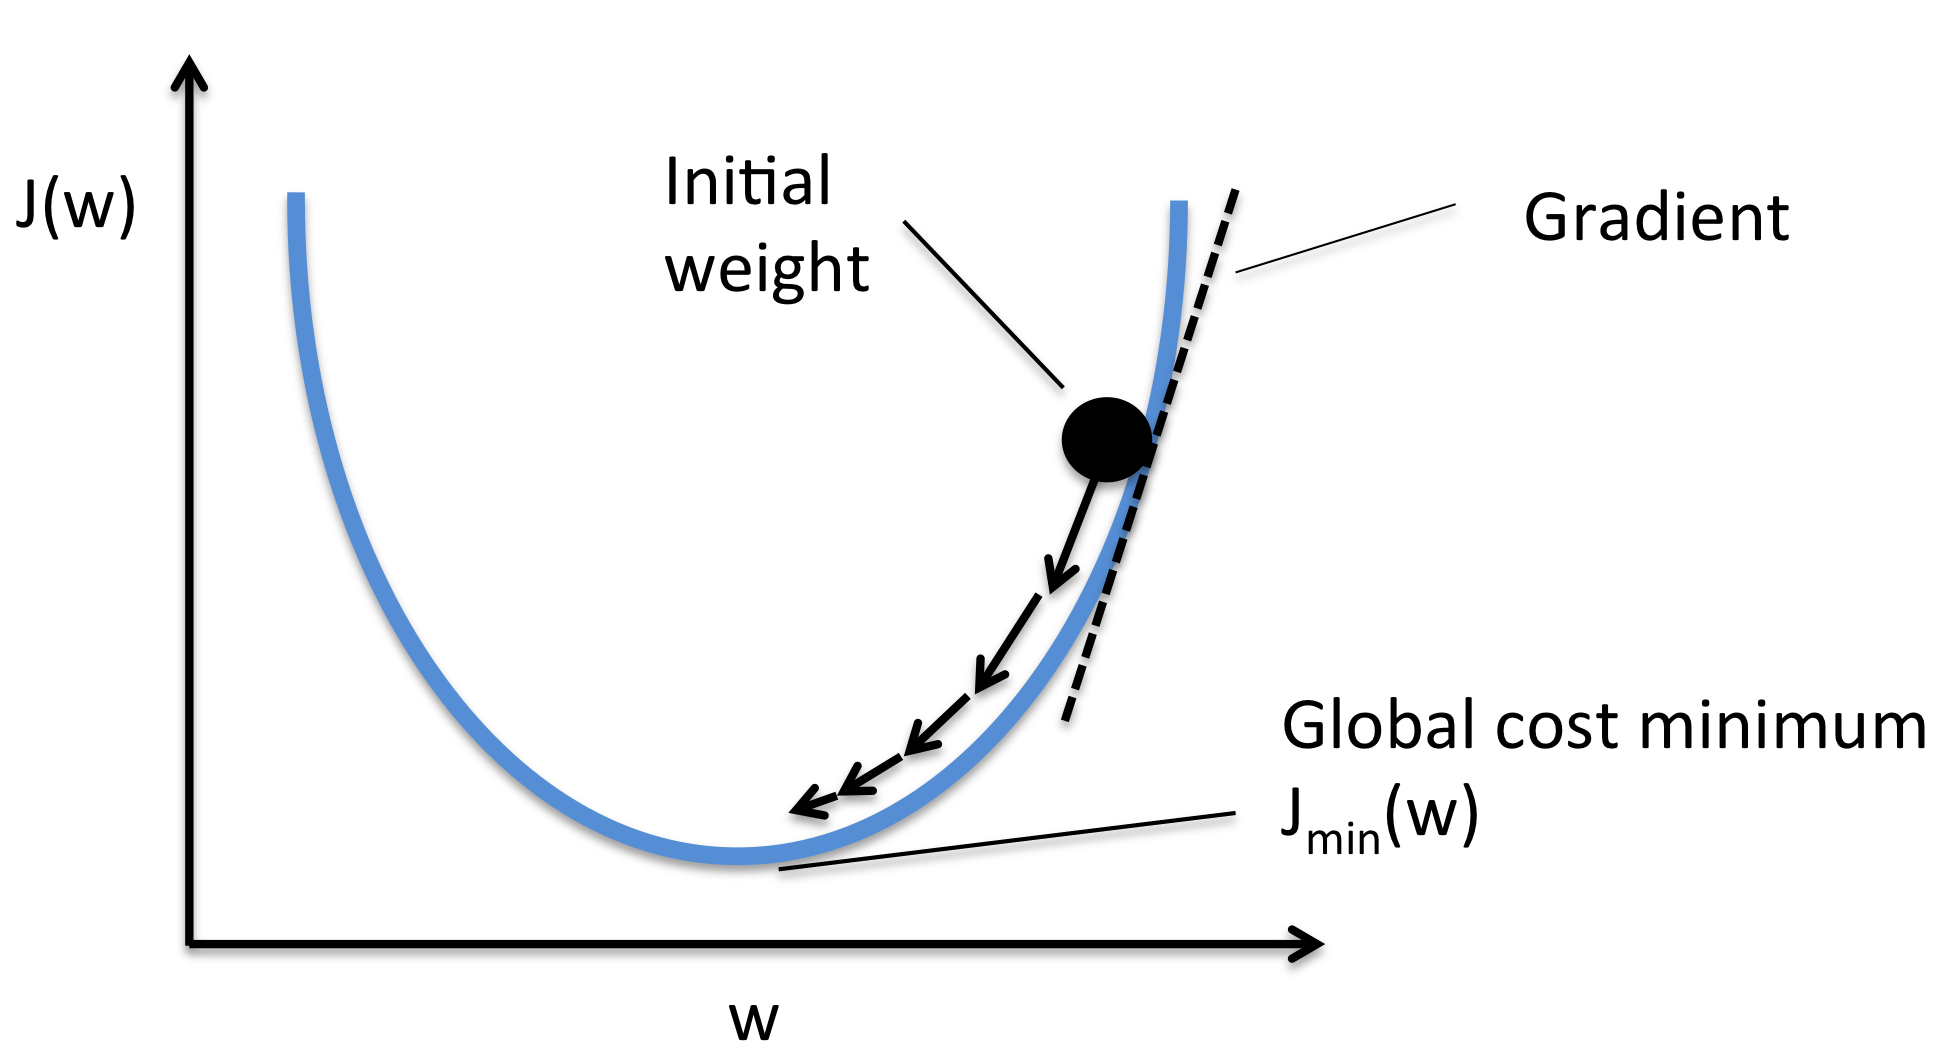
\includegraphics[scale=0.15]{pics/sgd.png}
\end{figure}
\footnotetext{Fuente: \url{https://sebastianraschka.com/images/faq/closed-form-vs-gd/ball.png}}

\begin{figure}[htb]
	\centering
	 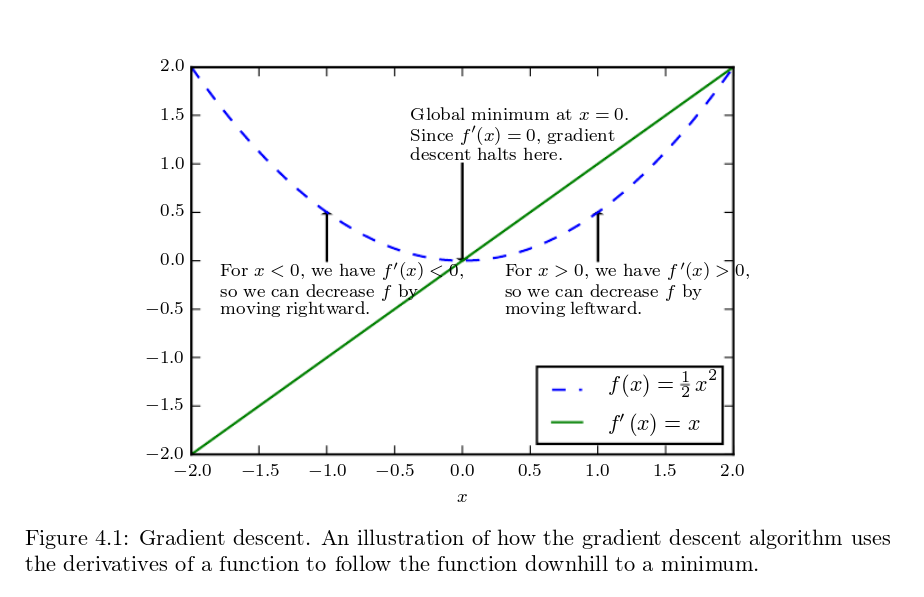
\includegraphics[scale=0.45]{pics/gradientdescent.png}
\end{figure}
\footnotetext{\cite{goodfellow2016deep}}

\subsection{Descenso de Gradiente Estocástico en Línea}
\begin{itemize}
\item Todos los parámetros se inicializan con valores aleatorios ($\Theta$).
\item Para cada ejemplo de entrenamiento $(x,y)$, calculamos la pérdida $L$ con los valores actuales de $\Theta$.
\item Luego actualizamos los parámetros con la siguiente regla hasta que se alcance la convergencia:
\item $\Theta_i \leftarrow \Theta_i - \eta \frac{\partial L}{\Theta_i}(\hat{y},y)$ (para todos los parámetros $\Theta_i$)
\end{itemize}

\begin{figure}[htb]
	\centering
	 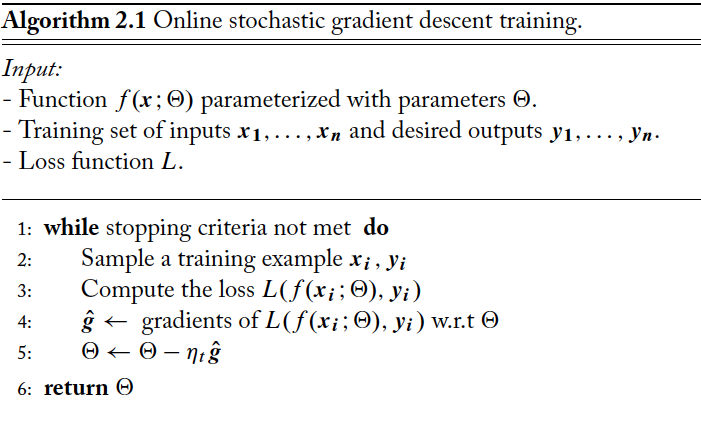
\includegraphics[scale=0.3]{pics/Online-SGD.png}
\end{figure}
\footnotetext{Fuente:\cite{goldberg2017neural}}

La tasa de aprendizaje puede ser fija durante todo el proceso de entrenamiento o puede decrecer como función del paso de tiempo $t$. El error calculado en la línea 3 se basa en un solo ejemplo de entrenamiento y, por lo tanto, es solo una estimación aproximada de la pérdida en todo el corpus $L$ que queremos minimizar. El ruido en el cálculo de la pérdida puede resultar en gradientes inexactos (los ejemplos individuales pueden proporcionar información ruidosa).

\subsection{Descenso de Gradiente Estocástico en Mini-batch}
\begin{itemize}
\item Una forma común de reducir este ruido es estimar el error y los gradientes en función de una muestra de $m$ ejemplos.
\item Esto da lugar al algoritmo de SGD en mini-batch.
\end{itemize}

\begin{figure}[htb]
	\centering
	 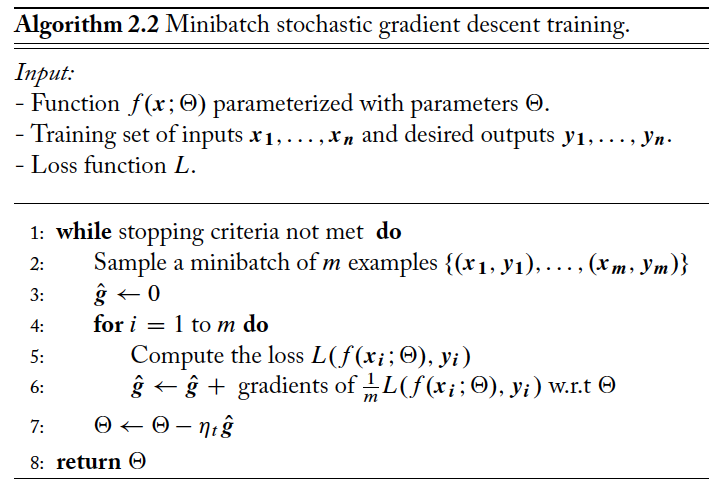
\includegraphics[scale=0.25]{pics/minibatch-SGD.png}
\end{figure}

Valores más altos de $m$ proporcionan mejores estimaciones de los gradientes en todo el corpus, mientras que valores más pequeños permiten más actualizaciones y, a su vez, una convergencia más rápida.

Para tamaños moderados de

$m$, algunas arquitecturas de cómputo (por ejemplo, GPUs) permiten una implementación paralela eficiente del cálculo en las líneas 3-6.

\footnotetext{Fuente:\cite{goldberg2017neural}}


%Translate this Latex book chapter to Spanish. Output in Latex format. Rearrange bullet points (\items) into full paragraphs. Make sure that sentences are connected in a more fluid way as they come.
\subsection{Funciones de Pérdida}
Las funciones de pérdida son utilizadas en algoritmos de aprendizaje automático para medir la discrepancia entre las predicciones del modelo y los valores reales de los datos de entrenamiento. Algunas funciones de pérdida comunes son:

\begin{itemize}
 \item Pérdida Hinge (o pérdida SVM): utilizada en problemas de clasificación binaria, donde la salida del clasificador es un escalar $\tilde{y}$ y la salida deseada $y$ está en el conjunto $\{+1,-1\}$. La regla de clasificación es $\hat{y} = \text{signo}(\tilde{y})$, y se considera una clasificación correcta si $y \cdot \tilde{y} > 0$. La función de pérdida se define como:
 \begin{displaymath}
  L_{\text{hinge(binaria)}}(\tilde{y},y) = \max(0,1-y \cdot \tilde{y})
 \end{displaymath}

 \item Entropía cruzada binaria (o pérdida logística): utilizada en clasificación binaria con salidas de probabilidad condicional. La salida del clasificador $\tilde{y}$ se transforma utilizando la función sigmoide para que esté en el rango $[0,1]$, y se interpreta como la probabilidad condicional $P(y=1|x)$. La función de pérdida se define como:
  \begin{displaymath}
  L_{\text{logística}}(\hat{y},y) = -y \log \hat{y} - (1-y) \log(1-\hat{y})
 \end{displaymath}

 \item La pérdida logística tiene una interpretación probabilística. Se asume que $P(y =1 | \vec{x} ; \Theta) = \sigma(f(\vec{x})) = \frac{1}{1+e^{-\vec{x}\cdot \vec{w}+b}}$ y $P(y = 0 | \vec{x} ; \Theta) = 1 - \sigma(f(\vec{x}))$. Esto se puede escribir de manera más compacta como:
 \begin{displaymath}
  P(y | \vec{x} ; \Theta) = \sigma(f(\vec{x}))^y\times(1-\sigma(f(\vec{x})))^{1-y}
 \end{displaymath}

 \item La expresión anterior es la función de masa de probabilidad de la distribución de Bernoulli.

 \item Si reemplazamos $\sigma(f(\vec{x}))$ por $\hat{y}$, obtenemos:
 \begin{displaymath}
  P(y | \vec{x} ; \Theta) = \hat{y}^y\times(1-\hat{y})^{1-y}
 \end{displaymath}
 \item Si aplicamos la estimación de máxima verosimilitud a esta expresión y tomamos el logaritmo, obtenemos:
 \begin{displaymath}
  y \log \hat{y} + (1-y) \log(1-\hat{y})
 \end{displaymath}

 \item ¡Maximizar esta expresión es equivalente a minimizar la pérdida logística!

 \item ¡Muchas funciones de pérdida corresponden al logaritmo negativo de la verosimilitud de modelos probabilísticos!



\item Pérdida de entropía cruzada categórica: se utiliza cuando se desea una interpretación probabilística de las puntuaciones de múltiples clases. Mide la discrepancia entre la distribución de etiquetas reales $\vec{y}$ y la distribución de etiquetas predichas $\vec{\hat{y}}$. La función de pérdida se define como:
\begin{displaymath}
L_{\text{entropía cruzada}}(\vec{\hat{y}},\vec{y}) = - \sum_{i} \vec{y}_{[i]} \log(\vec{\hat{y}}_{[i]})
\end{displaymath}

\item Cuando se utiliza la pérdida de entropía cruzada, se asume que la salida del clasificador se transforma utilizando la función softmax.

\item La función softmax comprime la salida de $k$ dimensiones a valores en el rango (0,1) de modo que todas las entradas sumen 1. Por lo tanto, $\vec{\hat{y}}_{[i]} = P(y = i |x)$ representa la distribución de pertenencia a la clase condicional.

\item Para problemas de clasificación dura en los que cada ejemplo de entrenamiento tiene una única asignación de clase correcta, $\vec{y}$ es un vector one-hot que representa la clase verdadera. En tales casos, la entropía cruzada se simplifica a:
\begin{displaymath}
L_{\text{entropía cruzada (clasificación dura)}}(\vec{\hat{y}},\vec{y}) = -\log(\vec{\hat{y}}_{[t]})
\end{displaymath}
donde $t$ es la asignación de clase correcta.

\end{itemize}

\section{Regularización}
Nuestro problema de optimización puede tener múltiples soluciones y, especialmente en dimensiones más altas, puede sufrir de sobreajuste. Consideremos el siguiente escenario en nuestro problema de identificación de idioma: uno de los documentos en el conjunto de entrenamiento ($\vec{x}_O$) es un valor atípico. En realidad, el documento está en alemán, pero está etiquetado como francés.

Para reducir la pérdida, el modelo puede identificar características (bigramas de letras) en $\vec{x}_O$ que ocurren en pocos otros documentos. El modelo asignará a estas características pesos muy altos hacia la clase francesa (incorrecta). Esto es una solución incorrecta para el problema de aprendizaje, ya que el modelo está aprendiendo algo incorrecto. Los documentos alemanes que comparten muchas palabras con $\vec{x}_O$ podrían clasificarse erróneamente como franceses. Nos gustaría controlar estos casos y alejar al modelo de soluciones equivocadas.

La idea de la regularización es agregar un término de regularización $R$ al objetivo de optimización. El objetivo de este término es controlar la complejidad (pesos grandes) del valor de los parámetros ($\Theta$) y evitar el sobreajuste:

\begin{equation}
\begin{split}
\hat{\Theta} \quad & = \operatorname{argmin}_{\Theta} \mathcal{L}(\Theta) + \lambda R(\Theta) \\
\quad & = \operatorname{argmin}_{\Theta} \frac{1}{n} \sum_{i=1}^n L(f(\vec{x}_i;\Theta), y_i) + \lambda R(\Theta) \\
\end{split}
\end{equation}

El término de regularización considera los valores de los parámetros y evalúa su complejidad. El valor del hiperparámetro $\lambda$ debe establecerse manualmente en función del rendimiento de clasificación en un conjunto de desarrollo.

En la práctica, los regularizadores $R$ consideran la complejidad como pesos grandes. Trabajan para mantener los valores de los parámetros ($\Theta$) bajos. Las opciones comunes para $R$ son la norma $L_2$, la norma $L_1$ y la elastic-net.

\subsection{Regularización L$_2$}
En la regularización $L_2$, $R$ toma la forma de la norma al cuadrado $L_2$ de los parámetros. El objetivo es mantener baja la suma de los cuadrados de los valores de los parámetros:

\begin{displaymath}
R_{L_{2}}(W) = ||W||^{2}_{2} = \sum_{i,j}(W_{[i,l]})^2
\end{displaymath}

El regularizador $L_2$ también se llama una priori gaussiana o decaimiento de peso. Los modelos regularizados con $L_2$ se ven severamente penalizados por pesos de parámetros altos. Una vez que el valor está lo suficientemente cerca de cero, su efecto se vuelve insignificante. El modelo preferirá disminuir el valor de un parámetro con peso alto en 1 en lugar de disminuir el valor de diez parámetros que ya tienen pesos relativamente bajos en 0.1 cada uno.

\subsection{Regularización L$_1$}
En la regularización $L_1$, $R$ toma la forma de la norma $L_1$ de los parámetros. El objetivo es mantener baja la suma de los valores absolutos de los parámetros:

\begin{displaymath}
R_{L_{1}}(W) = ||W||_{1} = \sum_{i,j} |W_{[i,l]}|
\end{displaymath}

A diferencia de $L_2$, el regularizador $L_1$ se penaliza de manera uniforme para valores bajos y altos. Tiene incentivos para disminuir todos los valores de parámetros no nulos hacia cero. Por lo tanto, fomenta soluciones dispersas, es decir, modelos con muchos parámetros con valor cero. El regularizador $L_1$ también se llama una priori dispersa o lasso \cite{tibshirani1996regression}.

\subsection{Elastic-Net}
El método de regularización elastic-net \cite{zou2005regularization} combina tanto la regularización $L_1$ como la regularización $L_2$ de la siguiente manera:

\begin{displaymath}
R_{\text{elastic-net}}(W) = \lambda_1 R_{L_1}(W) + \lambda_2 R_{L_2}(W)
\end{displaymath}


\section{Más allá del SGD}
Aunque el algoritmo SGD puede producir buenos resultados, también existen algoritmos más avanzados disponibles. Los algoritmos SGD+Momentum \cite{polyak1964some} y Nesterov Momentum \cite{nesterov2018lectures,sutskever2013importance} son variantes de SGD en las que los gradientes anteriores se acumulan y afectan la actualización actual. Los algoritmos de tasa de aprendizaje adaptativa, como AdaGrad \cite{duchi2011adaptive}, AdaDelta \cite{zeiler2012adadelta}, RMSProp \cite{tieleman2012lecture} y Adam \cite{kingma2014adam}, están diseñados para seleccionar la tasa de aprendizaje para cada minibatch. A veces, esto se hace de manera individual por coordenada, lo que puede aliviar la necesidad de ajustar la programación de la tasa de aprendizaje. Para obtener más detalles sobre estos algoritmos, consulte los documentos originales o \cite{goodfellow2016deep} (Secciones 8.3, 8.4).


\section{Conjuntos de entrenamiento, prueba y validación}
Cuando entrenamos un modelo, nuestro objetivo es producir una función $f(\vec{x})$ que mapee correctamente las entradas $\vec{x}$ a las salidas $\hat{y}$ según lo evidenciado por el conjunto de entrenamiento. La evaluación del rendimiento en los datos de entrenamiento puede ser engañosa, ya que nuestro objetivo es entrenar una función capaz de generalizar a ejemplos no vistos. Una forma común de abordar esto es dividir el conjunto de entrenamiento en subconjuntos de entrenamiento y prueba (80\% y 20\% respectivamente). Se entrena el modelo en el subconjunto de entrenamiento y se calcula la precisión en el subconjunto de prueba.

Sin embargo, este enfoque tiene una limitación. En la práctica, a menudo se entrenan varios modelos, se comparan sus calidades y se selecciona el mejor. Si se selecciona el mejor modelo en función de la precisión en el subconjunto de prueba, se obtendrá una estimación excesivamente optimista de la calidad del modelo. No se sabe si la configuración elegida del clasificador final es buena en general o simplemente es buena para los ejemplos particulares en los subconjuntos de prueba.

La metodología aceptada es utilizar una división de tres vías de los datos en conjuntos de entrenamiento, validación (también llamado desarrollo) y prueba\footnote{Un enfoque alternativo es la validación cruzada, pero no se escala bien para entrenar redes neuronales profundas.}. Esto proporciona dos conjuntos apartados: un conjunto de validación (también llamado conjunto de desarrollo) y un conjunto de prueba. Todos los experimentos, ajustes, análisis de errores y selección de modelos deben realizarse

basados en el conjunto de validación. Luego, una única ejecución del modelo final sobre el conjunto de prueba proporcionará una buena estimación de su calidad esperada en ejemplos no vistos. Es importante mantener el conjunto de prueba lo más limpio posible, realizando la menor cantidad de experimentos posible en él. Incluso algunos defienden que no se deben mirar siquiera los ejemplos en el conjunto de prueba, para evitar sesgar el diseño del modelo.

\begin{figure}[htb]
	\centering
	 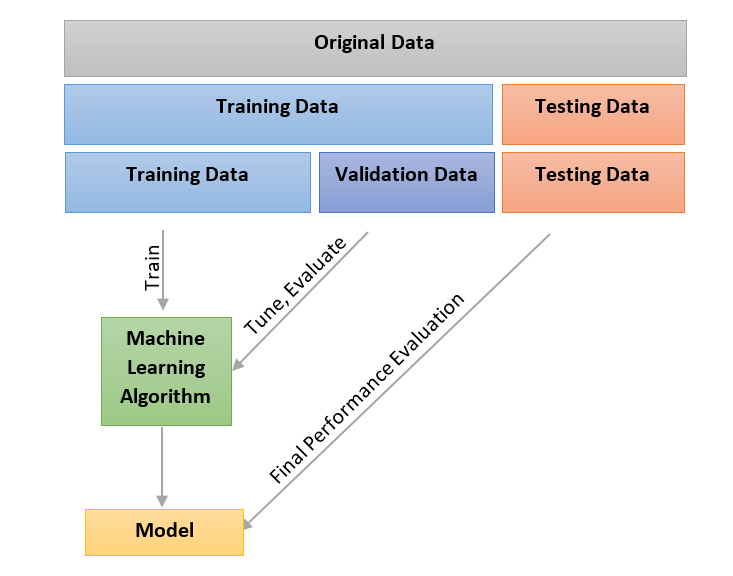
\includegraphics[scale=0.55]{pics/validation.png}
\end{figure}

\footnotetext{Fuente: \url{https://www.codeproject.com/KB/AI/1146582/validation.PNG}}


\section{Una limitación de los modelos lineales: el problema XOR}
La clase de hipótesis de modelos lineales (y log-lineales) está severamente restringida. Por ejemplo, no puede representar la función XOR, definida como:

\begin{equation}
\begin{split}
\operatorname{xor}(0,0) \quad & = 0 \\
\operatorname{xor}(1,0) \quad & = 1 \\
\operatorname{xor}(0,1) \quad & = 1 \\
\operatorname{xor}(1,1) \quad & = 0 \\
\end{split}
\end{equation}

No existe una parametrización $\vec{w} \in \mathbb{R}^2, b \in \mathbb{R}$ tal que:

\begin{equation}
\begin{split}
(0,0) \cdot \vec{w} + b \quad & < 0 \\
(0,1) \cdot \vec{w} + b \quad & \geq 0 \\
(1,0) \cdot \vec{w} + b \quad & \geq 0 \\
(1,1) \cdot \vec{w} + b \quad & < 0 \\
\end{split}
\end{equation}

Para ver por qué, consideremos el siguiente gráfico de la función XOR, donde los Os azules denotan la clase positiva y las X verdes la clase negativa.

\begin{figure}[htb]
	\centering
	 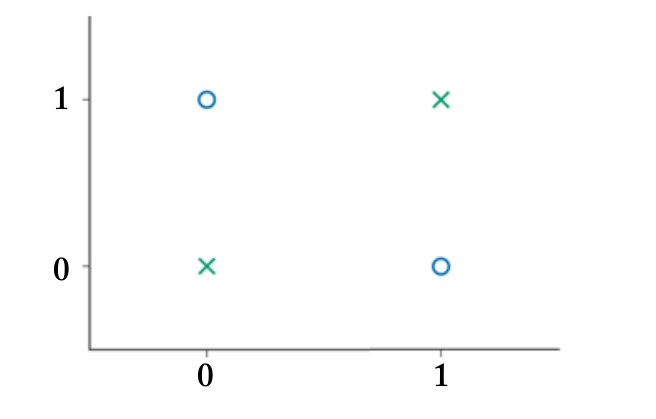
\includegraphics[scale=0.35]{pics/xor.png}
\end{figure}

Es evidente que ninguna línea recta puede separar las dos clases.


\subsection{Transformaciones no lineales de las entradas}
Si transformamos los puntos alimentándolos a través de la función no lineal $\phi(x_1,x_2) = [x_1 \times x_2, x_1 + x_2]$, el problema XOR se vuelve linealmente separable.

\begin{figure}[htb]
	\centering
	 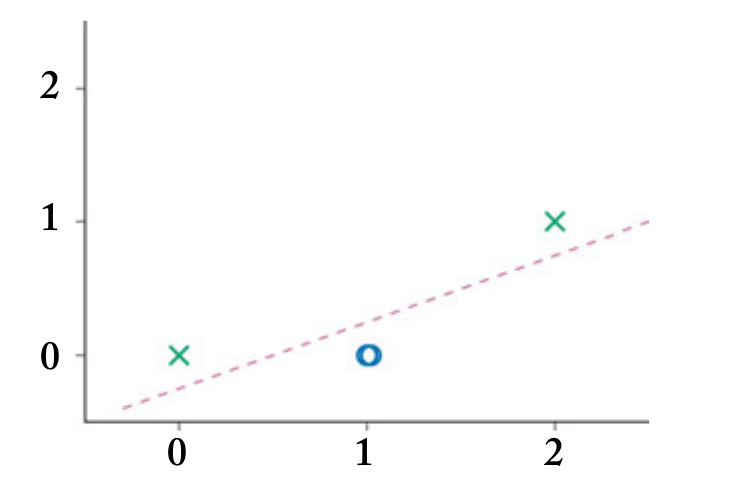
\includegraphics[scale=0.25]{pics/xor2.png}
\end{figure}

La función $\phi$ mapea los datos a una representación adecuada para la clasificación lineal. Ahora podemos entrenar fácilmente un clasificador lineal para resolver el problema XOR.

\begin{equation}
\hat{y} = f(\vec{x}) = \phi(\vec{x}) \cdot \vec{w} + b
\end{equation}

El problema es que necesitamos definir manualmente la función $\phi$. Este proceso depende del conjunto de datos particular y requiere mucha intuición humana. La sol

ción es definir una función de mapeo no lineal entrenable y entrenarla junto con el clasificador lineal. Encontrar la representación adecuada se convierte en responsabilidad del algoritmo de entrenamiento.

Las funciones de mapeo pueden tomar la forma de un modelo lineal parametrizado, seguido de una función de activación no lineal $g$ que se aplica a cada una de las dimensiones de salida:

\begin{equation}
\begin{split}
\hat{y} = f(\vec{x}) = \phi(\vec{x}) \cdot \vec{w} + b \\
\phi(\vec{x}) = g(\vec{x}W' + \vec{b}') \\
\end{split}
\end{equation}

Si tomamos $g(x) = \operatorname{max}(0, x)$ y $W' = \begin{pmatrix}
    1 & 1 \\ 1 & 1 \end{pmatrix}$, $\vec{b}' = \begin{pmatrix}
    -1 & 0 \end{pmatrix}$, obtenemos un mapeo equivalente a $[x_1 \times x_2, x_1 + x_2]$ para nuestros puntos de interés (0,0), (0,1), (1,0) y (1,1). ¡Esto resuelve con éxito el problema XOR!

Aprender tanto la función de representación como el clasificador lineal en la parte superior de ella al mismo tiempo es la idea principal detrás del aprendizaje profundo y las redes neuronales. De hecho, la ecuación anterior describe una arquitectura de red neuronal muy común llamada perceptrón multicapa (MLP, por sus siglas en inglés).
